\chapter{Gebruikte technologie}
Om de thesis tot een goed einde te brengen, werd gebruik gemaakt van een aantal bestaande technologieën. In wat volgt wordt een korte introductie gegeven met betrekking tot deze technologieën. Eerst worden de gehanteerde mobiele toestellen toegelicht waarna een korte uiteenzetting volgt van de ingebouwde sensoren. Vervolgens komen de gebruikte software \textit{libraries} en \textit{APIs} aan bod.

\section{Mobiele toestellen}
\subsection{Polar M600} \label{polar}
De Polar M600 is een smartwatch die Wear OS en de sportfuncties van polar samenbrengt. Het sporthorloge is compatibel met de meeste android \textit{smartphones} en iphones. Wear OS maakt het mogelijk om meldingen komende van de gekoppelde smartphone op de smartwatch te ontvangen alsook muziek en email communicatie te beheren. De Polar M600 (zie figuur \ref{fig:polarM600}) heeft een ingebouwde hartslagmeter wat nuttig is voor dit onderzoek.
Polar smartwatches kunnen gebruik maken van een aantal platformen voor visualisatie van trainingsdata \cite{ref24}. 
De Polar beat applicatie wordt onder andere gebruikt om data gegeneerd door de Polar toestellen te exporteren naar CSV formaat. Deze data is beschikbaar onder twee vormen: session data en \textit{raw data}. Session data bestaat uit de hartslag, de tijd in iedere hartslagzone, de afstand, de snelheid, afstand in iedere snelheidszone, \textit{training load} en herstelperiode. Onbewerkte data daarentegen bestaat uit het aantal samples per seconde, snelheid, afstand, versnelling en \textit{running cadence} \citep{ref8}. 
Met de polar M600 is het echter jammer genoeg niet mogelijk om de onbewerkte data te extraheren.
Polar flow is de web equivalent hiervan en biedt dezelfde functionaliteit als Polar beat \citep{ref9}. \\
Het assenstelsel van een smartwatch ziet eruit zoals op figuur \ref{fig:assenstelsel-smart}. Dit is nuttige info voor de analyse van accelerometer data.

\begin{figure}[!htpd]
\centering
\begin{floatrow}
  \ffigbox[\FBwidth]{\caption{Assenstelsel smartwatch \cite{ref74}}\label{fig:assenstelsel-smart}}{%
    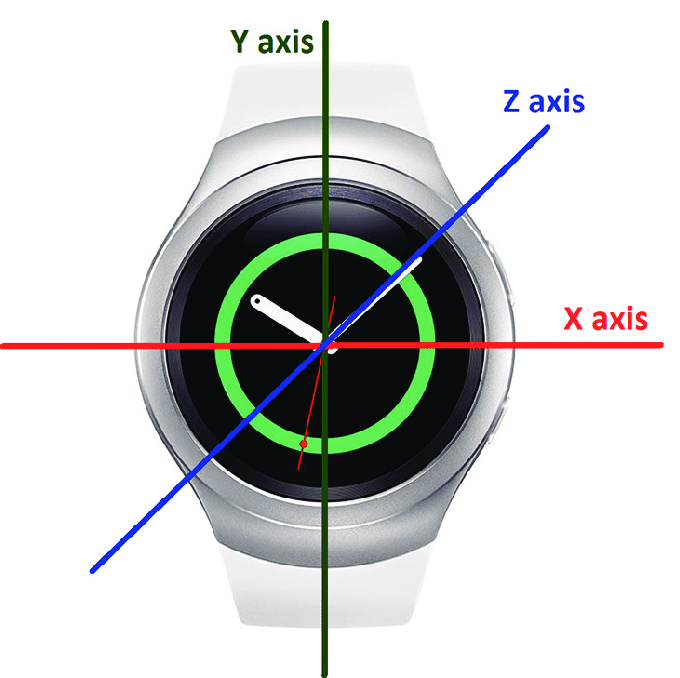
\includegraphics[width=0.5\textwidth]{apparatuur/Smartwatch-accelerometer-axes.png} 
  }
  \ffigbox[\FBwidth]{\caption{Polar M600  \cite{ref24}}\label{fig:polarM600}}{%
    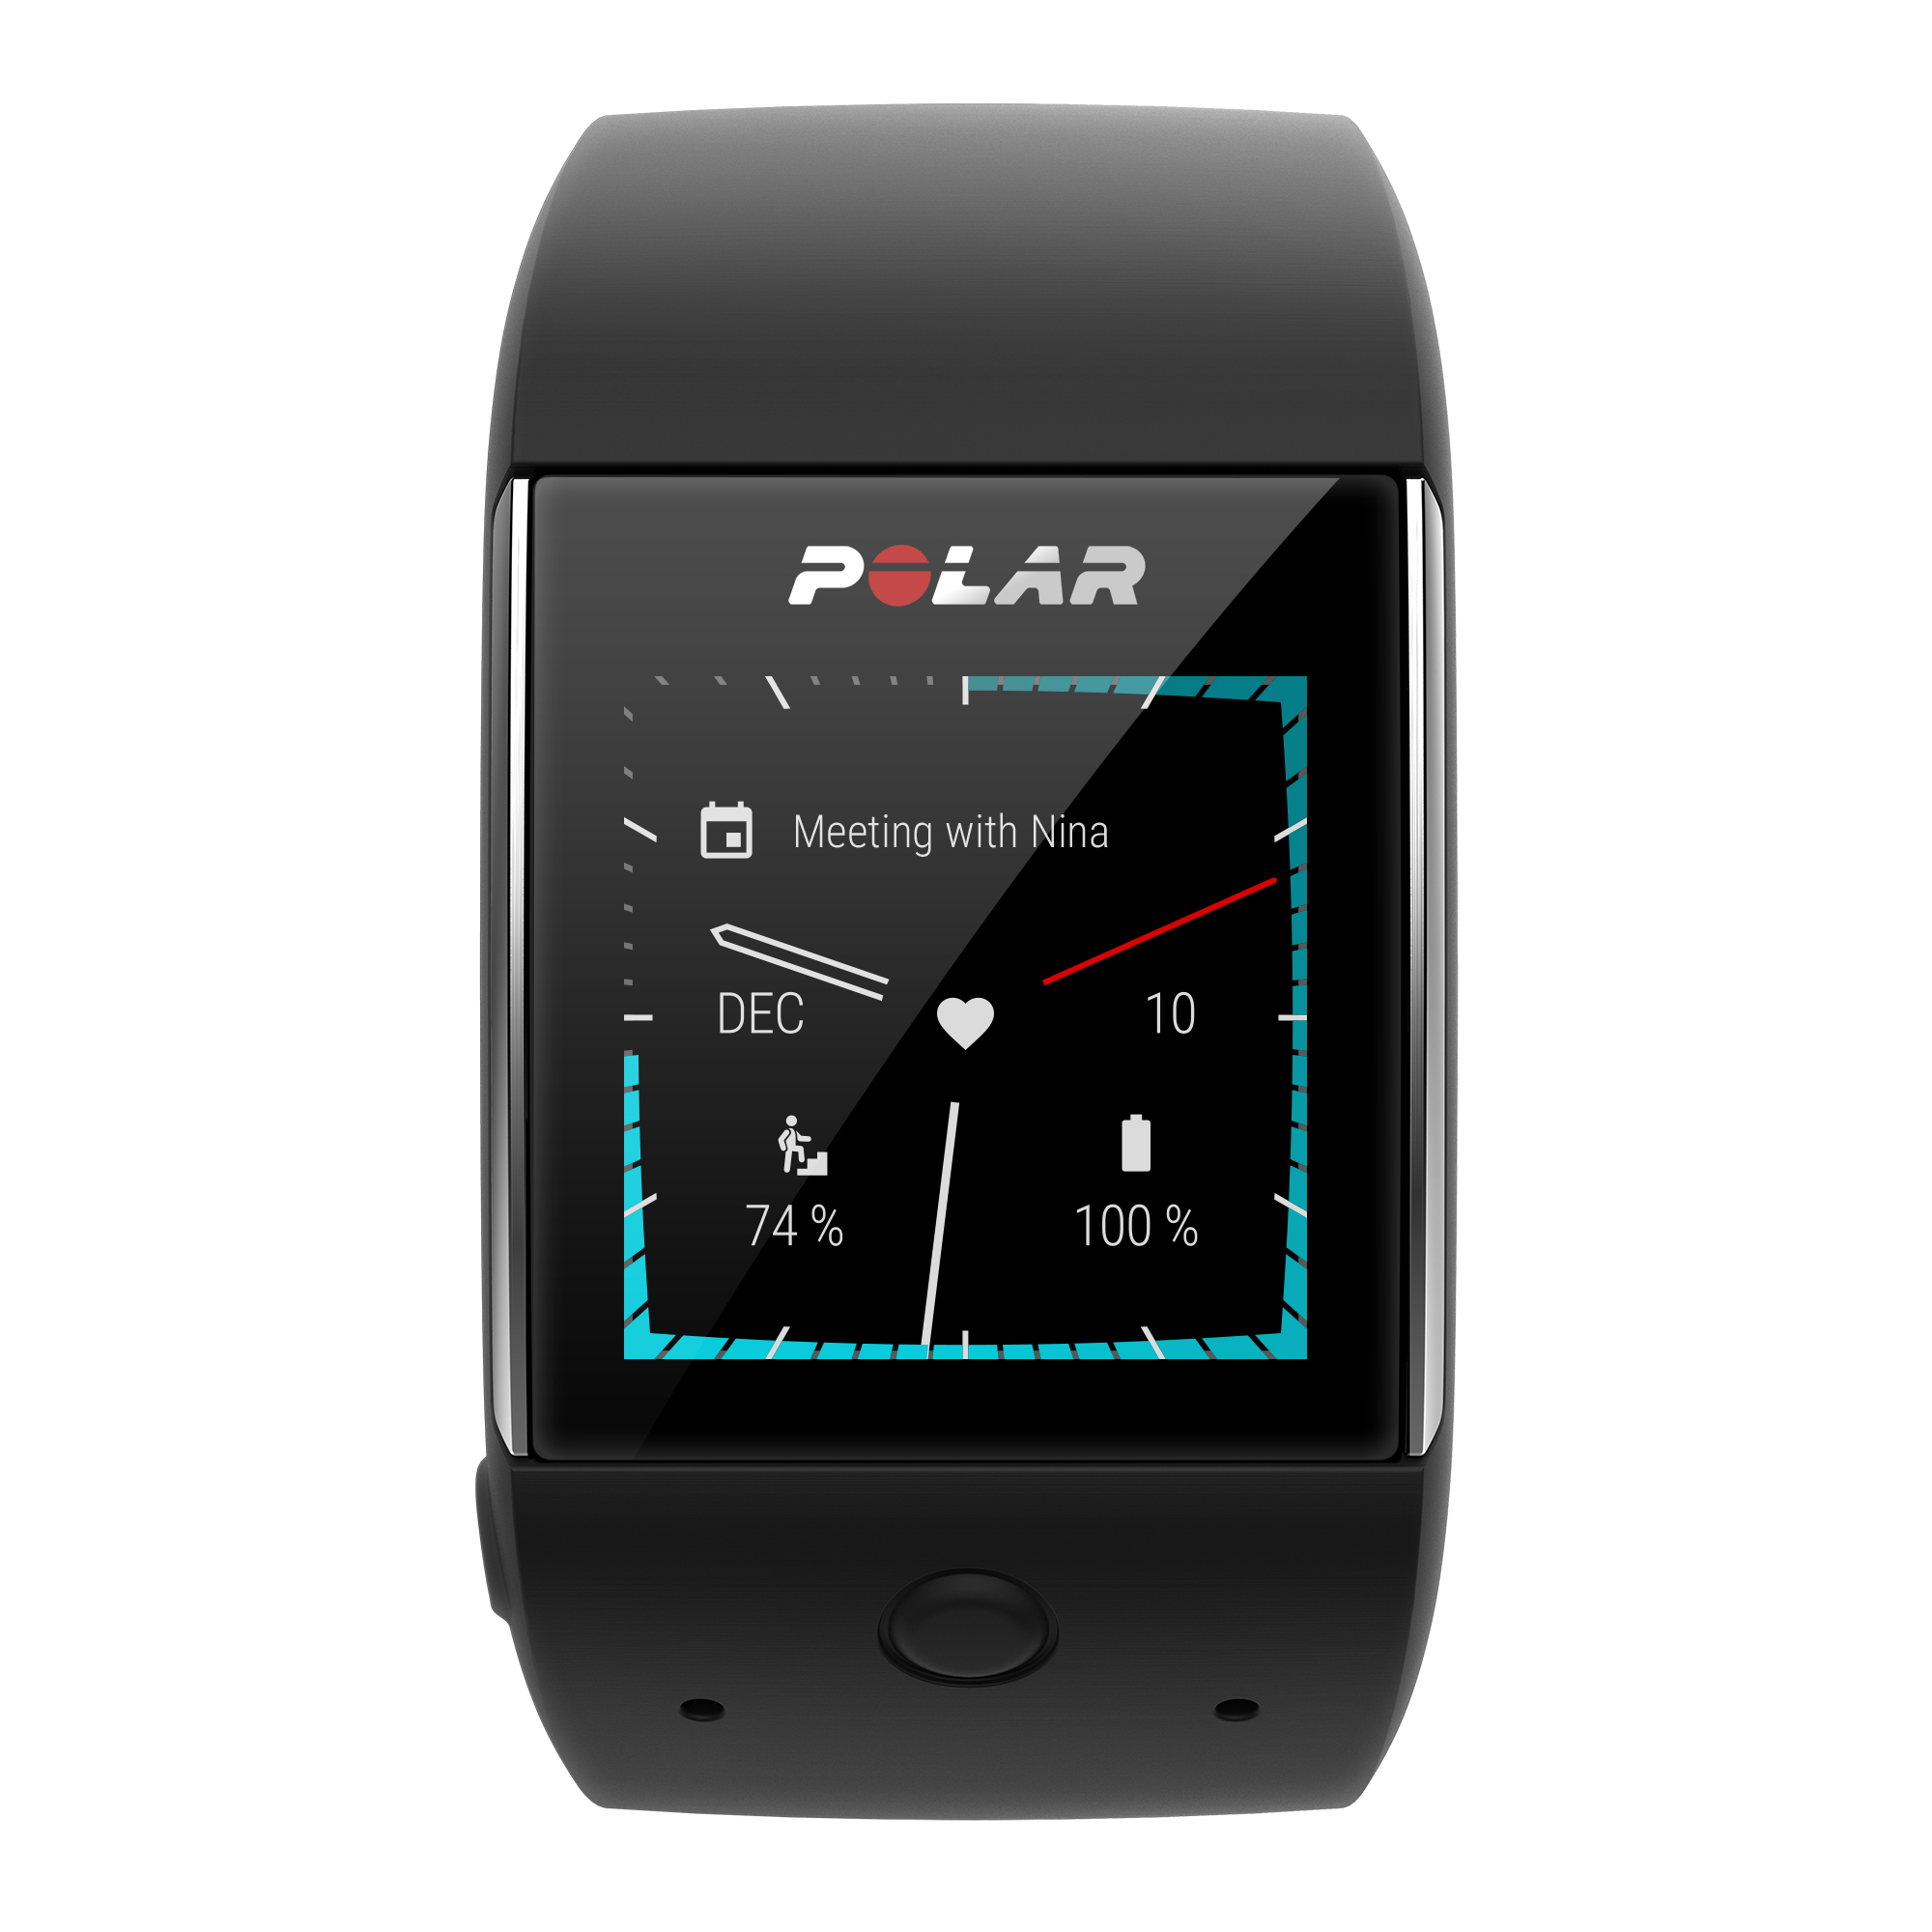
\includegraphics[width=0.5\textwidth]{apparatuur/polarM600.jpg}
  }
\end{floatrow}
\end{figure}

\subsection{Android smartphone}
Tijdens dit onderzoek werd gebruik gemaakt van een Huawei Nova voor het ontwikkelen en testen van de uiteindelijke applicatie alsook tijdens het data verzamelingsproces.  

\section{Sensoren}
Voor het herkennen van beweging is bepaalde data nodig afkomstig van sensoren. Ook is de bepaling van persoonlijke aanbevelingen afhankelijk van hartslagdata eveneens afkomstig van een sensor. Om deze redenen worden de gebruikte sensoren en hun interne werking kort toegelicht.

\subsection{Accelerometer}
Een accelerometer is een sensor gebruikt om versnellingskrachten in kaart te brengen. Deze krachten kunnen zowel statisch, zoals de zwaartekracht, als dynamisch zijn. 
Via kristalstructuren, die gespannen worden onder dwang van versnellingskrachten, wordt een voltage niveau gecreëerd. Via deze waarde is het mogelijk om een oriëntatie en lengte van de corresponderende vector te bepalen \cite{ref54}. Dit proces is te zien op figuur \ref{fig:werkingacc}

In android toestellen wordt typisch met twee verschillende coördinaat systemen gewerkt. Een eerste is een coördinaat stelsel relatief ten opzichte van het toestel. Een tweede vorm is een assenstelsel georiënteerd volgens de aarde.
De android accelerometer sensor gebruikt een 3D assenstelsel georiënteerd volgens de eerste manier, dus ten opzichte van het toestel. In dit soort coördinaten systeem worden de assen niet aangepast bij rotatie van het toestel.
De accelerometer sensor meet de versnelling langs elk van de assen al dan niet samen met de zwaartekracht, afhankelijk van het type sensor. De sensor met type TYPE\_LINEAR\_ACCELERATION houdt geen rekening met de bijdrage van de zwaartekracht. Het type TYPE\_GRAVITY kijkt dan weer enkel naar de zwaartekracht. 
De accelerometer sensor is zeer energiezuinig ten opzichte van andere sensoren wat een groot voordeel is bij langdurig gebruik \cite{ref55}.

\begin{figure}
\centering
\caption{Werking accelerometer \cite{ref56}}\label{fig:werkingacc}
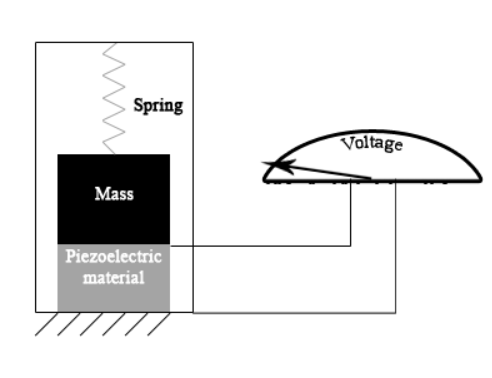
\includegraphics[scale=0.8]{apparatuur/accelerometer_spring.PNG}
\end{figure} 

\subsection{Hartslag sensor}
De Polar M600 utiliseert een optische sensor om hartslag te meten. Hierbij wordt gebruik gemaakt van licht om de bloedcirculatie in beeld te brengen. Een groen licht schijnt op de pols tijdens het meten. Verschillende golflengtes van deze lichtgolf interageren met het bloed. Het uitgezonden licht reflecteert hierop waarna een tweede sensor deze informatie, namelijk het al dan niet reflecteren van de lichtbundel, opvangt \cite{ref57}.

Wanneer bloed circuleert verandert namelijk het volume naarmate meer of minder circulatie aanwezig is. Licht zal minder goed reflecteren indien het bloedvolume hoog is. De tijd tussen lage en hoge gereflecteerde lichtintensiteit wordt gebruikt om de hartslag te berekenen \cite{ref58}. Figuur \ref{fig:hartslagsensor} visualiseert dit proces.

\begin{figure}
\centering
\caption{Werking hartslag sensor \cite{ref59}}\label{fig:hartslagsensor}
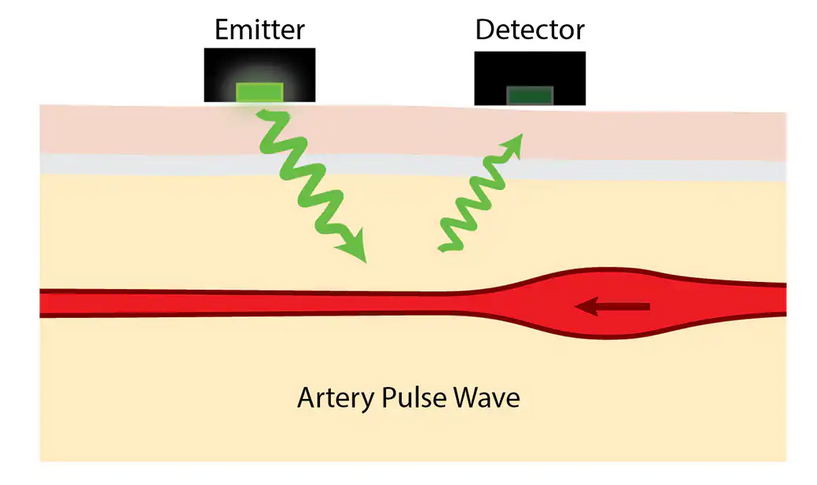
\includegraphics[scale=0.7]{apparatuur/heartrate_emitter.PNG}
\end{figure} 

\section{Software}
Volgende sectie beschrijft de gebruikte \textit{software libraries} en APIs. Hierbij zullen alle technologieën aan bod komen waarmee deze thesis in aanraking gekomen is. Ook zal telkens de reden voor het al dan niet gebruik ervan aangehaald worden.

\subsection{Google fit}
Google fit is een centrale opslagplaats voor fitnessdata waarbij interactie met meerdere applicaties mogelijk is.
De \textit{cloud service} bestaat uit een aantal componenten. Via de Google fit APIs kunnen verschillende high level representaties van elementen bekomen worden. Werken met de Fitstore is hierdoor gemakkelijk. Data Sources zijn één van deze \textit{high level} representaties, deze stellen sensoren voor. Data Types, een andere high level representatie, bevatten info over het soort data (aantal stappen, hartslag...). Data Points is een array van waarden met een bepaald data type, komende vanuit een data source. Datasets zijn datapunten van hetzelfde type van dezelfde source binnen een bepaald tijdsinterval. Sessions, als laatste, stellen een tijdsinterval voor waarin de gebruiker een activiteit beoefent. 
Omdat Google fit omgaat met vertrouwelijke fitness data en deze het toestel verlaat, is toestemming van de gebruiker noodzakelijk \citep{ref10}. \\

\noindent
Er werd gekozen om geen gebruik te maken van Google fit omwille van volgende redenen. Voor de detectie en aanbeveling van activiteiten wordt gebruik gemaakt van een eigen \textit{machine learning model}. Om interactie met Google fit mogelijk te maken zou dus een externe backend server noodzakelijk zijn. 
Ook zal vertrouwelijke fitnessdata het toestel moeten verlaten indien voor Google fit gekozen wordt. 
Google fit is afhankelijk van een werkende internetconnectie om recente data te kunnen weergeven. Een fitness applicatie ontwikkeld om de gebruiker optimaal te stimuleren baat echter voordeel bij een onafhankelijkheid van internet om resultaten in beeld te brengen.

\subsection{Scikit learn}
Scikit learn is een machine learning library voor python. Hierin zijn diverse algoritmes geïmplementeerd voor onder andere classificatie, regressie en unsupervised learning. Ook is het mogelijk om de aangeboden preprocessing functionaliteit te hanteren. Dit bevat onder andere normalisatie implementaties en standaard schalers. Eveneens zijn algoritmes die helpen bij de automatisering van alle stappen in het data analyse proces aanwezig (dimensionality reduction, Feature selection, feature extraction en feature engineering) \cite{ref60}.

\subsection{Google SignIn}
In deze thesis wordt Google SignIn gebruikt als authenticatiemiddel. Via deze weg kan de gebruiker inloggen met zijn/haar Google account. Deze service behoort tot de Google APIs. Er moet hiervoor dus een Google API console project aangemaakt worden. Indien authenticatie met een backend server mogelijk moet zijn, is een OAuth 2.0 client ID vereist. Deze moet meegegeven worden met de Google SignIn opties. 

\subsubsection{OAuth}
OAuth 2.0 is het standaard protocol voor authorizatie van client en server. Dit protocol zorgt voor (gelimiteerde) toegang van \textit{third party} applicaties naar een backend server.
Er zijn vier rollen gedefinieerd in het OAuth protocol. De eerste is \textit{resource owner}, dit is de instantie die de informatie aanvraagt. \textit{Resource server} is de server die uw persoonlijke data beheert. Cliënt is de applicatie die toegang vraagt tot de server. Authorisation server is de server die \textit{access tokens} uitdeelt aan de diverse clients. De rol van resource en \textit{authorisation server} kan door dezelfde machine opgenomen worden. Er wordt gebruik gemaakt van access tokens en \textit{refresh tokens}. Een access token geeft de toegang en moet vertrouwelijk gehouden worden. Refresh tokens worden gebruikt om access token te vernieuwen aangezien deze een beperkte levensduur hebben \cite{ref25}.

\subsection{Wearable Data Layer API}
Met behulp van Wear OS kan een smartwatch direct communiceren met een netwerk zonder gekoppeld te zijn aan een mobiel toestel. Indien er een connectie met een smartphone tot stand gebracht is via bluetooth zal het netwerkverkeer geproxied worden langs deze weg. In het andere geval maakt de smartwatch gebruik van Wi-Fi en cellulaire netwerken.
De Wearable Data Layer API biedt een afzonderlijk communicatie kanaal tussen applicaties aan. 
De API bevat een aantal data objecten die communicatie mogelijk maken. Een Data Item slaat info op en zorgt voor automatische syncing tussen gsm en smartwatch. Een Asset zorgt voor verzending van binaire \textit{blobs} van data. Een MessageClient verzendt berichten, de twee apparaten moeten hiervoor geconnecteerd zijn. Een ChannelClient wordt gebruikt voor verzending van grotere bestanden \cite{ref26}.
Deze thesis maakt enkel gebruik van de messageClient. De informatie die zal verzonden worden via deze weg is namelijk niet van die omvang dat een channelClient noodzakelijk is. Ook is gebruik maken van Data Items niet optimaal. Deze objecten zijn namelijk bedoeld om grotere meer persistente info op te slaan, wat hier niet het geval is. Assets zijn eveneens minder geschikt aangezien ze vooral worden gebruikt om afbeeldingen over te dragen.

\subsection{Firebase}
Firebase is een NoSQL document georiënteerde databank, data wordt opgeslagen in documenten die samen zitten in collecties. De databank is bijgevolg schemaloos. De collecties en documenten worden impliciet gecreëerd \cite{ref61}.
Gebruik van Firebase als opslagplaats voor sensor data is zeer duur. Firebase is namelijk betalend indien een bepaalde dagelijkse limiet overschreden wordt. Voor de opslag van sessie berekeningen is dit eveneens niet zeer geschikt om dezelfde reden als Google fit. Er is namelijk een internetconnectie noodzakelijk om weergave van recente berekeningen mogelijk te maken.

\subsection{Pandas framework}
Pandas is een data analyse library voor python. Het maakt gebruik van \textit{dataframe} objecten voor data manipulatie. Deze datastructuur maakt het mogelijk om de data voor te stellen in rijen van observaties en kolommen van variabelen \cite{ref27}.

\subsection{Tensorflow}
Tensorflow is een end-to-end platform voor het bouwen en \textit{deployen} van Machine Learning modellen. Dit framework maakt het mogelijk om neurale netwerken te ontwikkelen met vele lagen. Voor het bouwen en trainen van deep learning modellen maakt Tensorflow gebruik van Keras \cite{ref62}.

\subsubsection{Tensorflow Lite}

Tensorflow Lite is een manier om machine learning modellen te deployen op mobiele toestellen. Via de Tensorflow lite converter wordt een model geschreven in python geconverteerd naar het LITE formaat. Wanneer dit lite model gedeployed is, kunnen voorspellingen gemaakt worden aan de hand van een interpreter. De voorspelde data moet van dezelfde vorm zijn als waarop het model getraind heeft. Deze info kan verkregen worden via de inputtensor. Er mogen slechts een selectief aantal primitieve types gebruikt worden als input. Sensor data heeft echter telkens een float type wat ondersteund wordt. 
Als output wordt een array van probabiliteiten teruggegeven waarin de indices overeenkomen met de labelindices van het model \cite{ref63}.

\subsection{Workmanager} \label{subsection:workmanager}
Workmanager wordt gebruikt om in de achtergrond taken uit te voeren die niet op één specifiek moment moeten gebeuren. Met andere woorden ze zijn uitstelbaar. Dit is nodig om ervoor te zorgen dat de taken op een zo efficiënt mogelijke manier kunnen uitgevoerd worden. Er kan bijvoorbeeld gewacht worden tot het mobiele toestellen oplaadt of totdat de accu boven een zekere waarde stijgt. Een eerste manier om zogenoemde \textit{workrequests} te definiëren is met een OneTimeWorkRequest. Dit soort \textit{request} zorgt ervoor dat de taak, na een optionele vertraging, zo snel mogelijk en zo efficiënt mogelijk uitgevoerd wordt. Een andere manier, optimaal voor taken die telkens opnieuw moeten gerealiseerd worden, is via een PeriodicWorkRequest. Hiermee wordt een interval gespecificeerd waarin de taak kan uitgevoerd worden. Indien een kleiner tijdsinterval gewenst is, kan gebruik gemaakt worden van een \textit{flexinterval}. Dit zorgt ervoor dat de taak niet op eender welk moment binnen het globale interval mag uitgevoerd worden, maar enkel binnen het flexinterval. Via een instantie van het WorkManager object kunnen de verschillende requests gequeued worden (zie figuur \ref{fig:periodicwork}). Het is eveneens mogelijk om een bepaalde unieke job te behouden of om deze telkens te vervangen door een nieuw exemplaar. Dit om te voorkomen dat verschillende instanties van eenzelfde taak aanwezig zijn \cite{ref64}.

Toegepast op deze thesis kan Workmanager zeker zijn nut bewijzen. De berekening van nieuwe aanbevelingen gebaseerd op additionele fitnessdata zal namelijk periodiek gebeuren. Een andere optie was om telkens de aanbevelingspagina gerefreshed wordt, alle berekeningen van nul te herbeginnen. Dit zou een bottleneck kunnen vormen voor het systeem, vandaar de keuze voor Workmanager.

\begin{figure}
\centering
\caption{PeriodicWorkRequest \cite{ref65}}\label{fig:periodicwork}
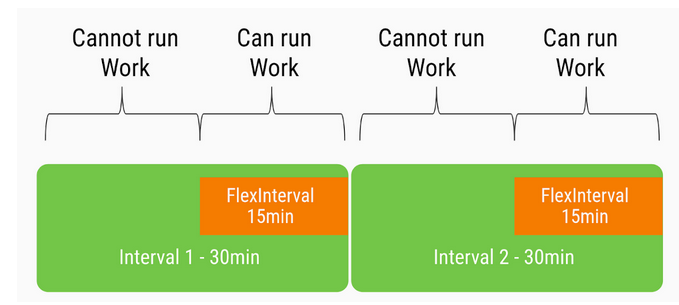
\includegraphics[scale=0.6]{apparatuur/periodicWorkRequest.PNG}
\end{figure} 

\subsection{Room}

De Room Persistence Library maakt onderliggend gebruikt van SQLite, maar biedt nog een extra abstractie laag voor gebruiksgemak. SQLite is een zeer kleine, \textit{lightweight database} waardoor het zicht zeer goed leent tot gebruik in mobiele toestellen. SQLite vereist ook geen speciale database server, het maakt gebruik van een filesysteem in SQL syntax \cite{ref66} \cite{ref67}.
Er werd gekozen voor een volledige lokale implementatie. Hierbij staat Room als opslagplaats centraal. De database wordt gebruikt om allerhande fitnessdata in te bewaren. Er zal rekening gehouden worden met de maximale capaciteit door tijdig historische data ouder dan tien weken te verwijderen. Dit heeft geen negatieve invloed op de werking van de applicatie aangezien deze ontworpen is voor een tien weken durende training.
